\documentclass[12pt,a4paper]{article}
\usepackage[pdfencoding=auto, colorlinks=false, pdfborder={0 0 0},pdftitle={Internship Report}, pdfauthor={Quentin Sonnefraud}, pdfsubject={Intership Report}, pdfkeywords={report, edf, Quentin, Sonnefraud, internship, angular, node.js, analytics, Epitech}, bookmarks=true, pdfcreator={Quentin Sonnefraud}, pdflang=US]{hyperref}
\usepackage[fencedCode,inlineFootnotes,citations,definitionLists,hashEnumerators,smartEllipses,hybrid]{markdown}
\usepackage{minted}
\usepackage{float}
\usepackage[english]{babel}
\usepackage{geometry}
\usepackage[utf8]{inputenc}
\usepackage[T1]{fontenc}
\usepackage{graphicx}
\usepackage{fancyhdr}
\usepackage{listings}
\usepackage{textcomp}
\usepackage{caption}
\usepackage[toc,xindy,nonumberlist]{glossaries}


%\geometry{dvips,a4paper,margin=1.5cm, top=1.5cm, bottom=2.5cm}

\def\title{Log Book}

\fancyhf{}
\fancyhead[L]{\textbf{\title}}
\fancyhead[R]{
\includegraphics[width=1.7cm]{assets/kent_logo.png}}
\fancyfoot[C]{\thepage}
\setlength{\headheight}{37pt}

\newcommand{\quickwordcount}[1]{%
  \immediate\write18{texcount -1 -sum -merge -q #1.tex output.bbl > #1-words.sum }%
  \input{#1-words.sum} words%
}



\author{Quentin Sonnefraud}
\date{1 April 2019 - 30 August 2019}

\setcounter{tocdepth}{4}
\setcounter{secnumdepth}{4}
\newcommand{\hsp}{\hspace{20pt}}
\newcommand{\HRule}{\rule{\linewidth}{0.5mm}}


\begin{document}
\thispagestyle{plain}
\begin{titlepage}
	\begin{sffamily}
		\begin{center}

			\begin{center}
				
\includegraphics[width=7cm]{assets/kent_logo.png}
			\end{center}
			\vspace{2cm}
			{\scshape\Large CO880: Project and Dissertation }\\[2cm]
			\HRule \\[0.4cm]
			{ \huge \bfseries \title \\[0.4cm] }
			\HRule \\[2cm]
			\bigskip
			\centering\LARGE{Quentin Sonnefraud} \\ \bigskip
			\Large{\today}


			\vfill
		\end{center}
	\end{sffamily}
\end{titlepage}

\pagebreak

\pagestyle{fancy}

\tableofcontents

\pagebreak

This document is about the work I have done for the dissertation project I first managed to understand the SQL data given by Stefan Marr for the project, and then in order to manipulate the data correctly, I wrapped the SQL backup in an API in order to be used by a jupyter notebook more easily.

All the engineering process can be followed at this address \url{https://github.com/Vatoth/master-thesis/commits/master}

\section{June 1st  - 7 June}
Exam are finished I'm starting the project, First meeting with Stefan Marr He explained me the project and the project RebenchDB, I'm looking a bit at the code, but I quickly realise that will spend to much time understanding the code of this project, I ask him a database backup in order to look at the data directly.

In order to manipulate the data quickly for the next week, I will develop a REST API.

First, I'm using node.js with typescript and with sequelize to map the database backup.

Sequelize is an ORM (Object Relational Mapping) which is responsible for translating the TypeScript object in SQL queries to save models.
I'm starting to add libraries:

$ npm install --save sequelize sqlite
$ npm install --save-dev r @ types / sequelize


Next, I will create a lib/config / database.ts file to configure Sequelize database system.

Then we can create a model for all table in the database. We will start with the Benchmark model which extends the Sequelize Model class:

\begin{lstlisting}
import {
  Column,
  PrimaryKey,
  AutoIncrement,
  Model,
  Table,
  AllowNull,
  DataType,
  HasMany,
  Unique,
} from "sequelize-typescript";
import { Run } from "./Run.model";

@Table({ tableName: "benchmark" })
export class Benchmark extends Model<Benchmark> {
  @AutoIncrement
  @PrimaryKey
  @Column(DataType.INTEGER)
  id: number;

  @AllowNull(true)
  @Unique
  @Column(DataType.STRING)
  name?: string;

  @AllowNull(true)
  @Column(DataType.STRING)
  description?: string;

  @HasMany(() => Run, "benchmarkid")
  runs: Run[];
}
\end{lstlisting}


Next, we configure the SQL schema for the table and call the Database.sync. This will create a table in the Postgresql database.

That's all! When I start it npm run dev server that table is automatically created.

\section{June 8 - June 14}

This week was about trying to understand the data and visualise it a bit. I'm making progress on changepoint analysis in order to understand it more, and I was doing wrong trying to compare between all segments of the measurement,

\begin{figure}[h]
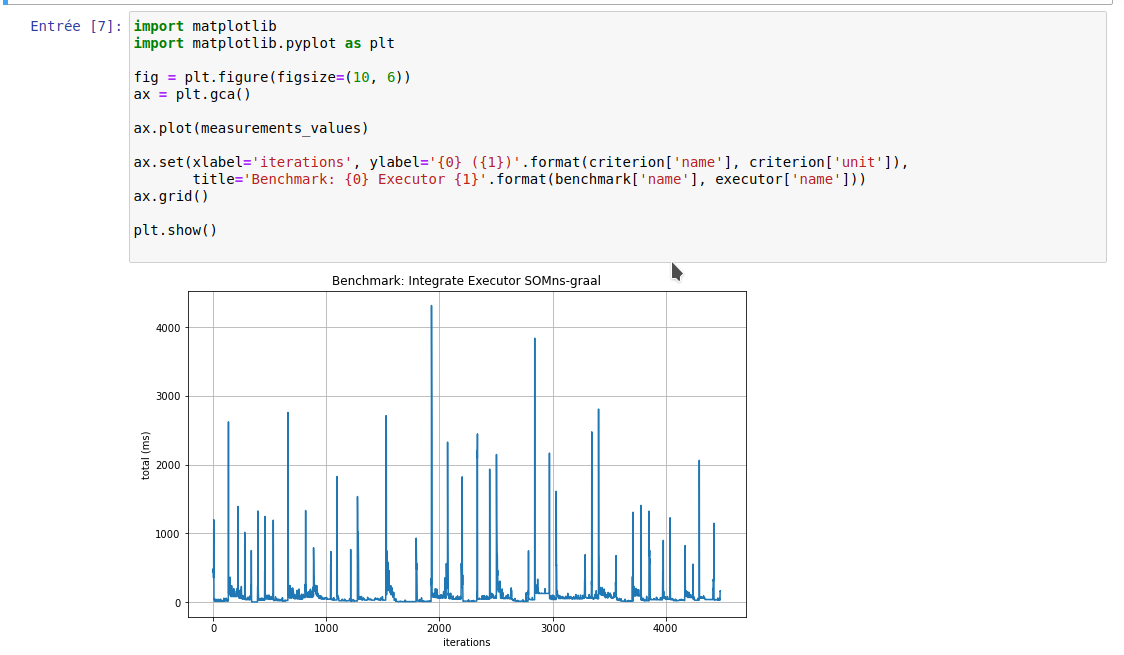
\includegraphics[width=8cm]{assets/Screenshot_20200906_111933.png}
\end{figure}


\begin{figure}[h]
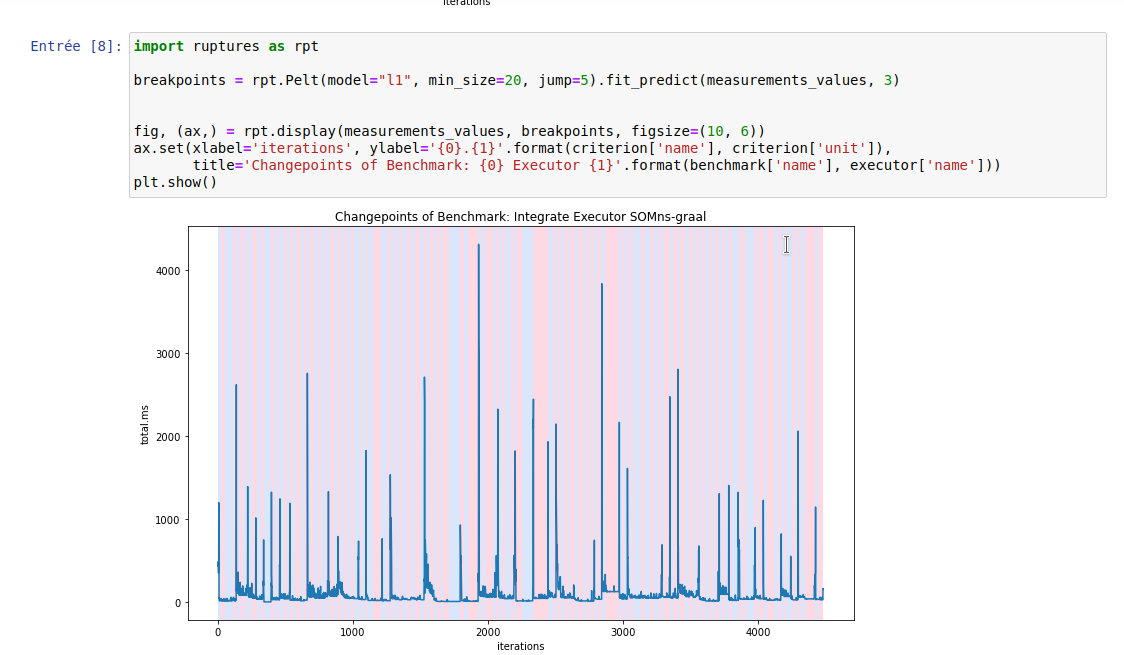
\includegraphics[width=8cm]{assets/Screenshot_20200906_111943.png}
\end{figure}


\begin{figure}[h]
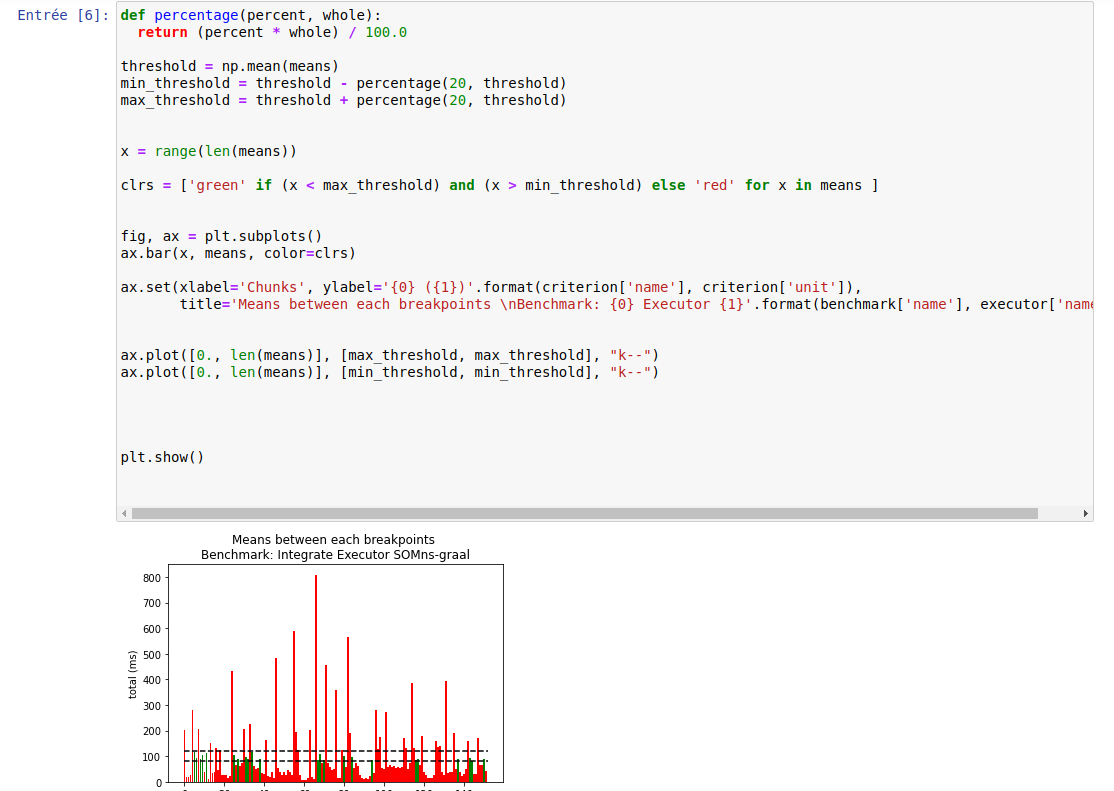
\includegraphics[width=8cm]{assets/Screenshot_20200906_112000.png}
\end{figure}


\section{June 14 - June 28}
This week was about the deployment of the project to use it and delegate some calculation on my server so I can I run the algorithm on my computer.


For the system implementation, I have used docker and docker-compose for the system administration and using Traefik for the load balancing and generating https certificate. 

So my understanding of  Docker Compose is a tool that allows to describe (in a YAML file) and manage (on the command line) several containers as a set of interconnected services.

\begin{itemize}

\item  Postgresql container which is a databases
\item  The api container with node.js
\item  Jupyter notebook to share my experiement and progress
\end{itemize}


\lstset{
  language=bash,
  basicstyle=\tiny
}

The next file is stack yml of my system.
\begin{lstlisting}
version: "3.3"

services:
  database:
    image: postgres
    environment:
      - POSTGRES_PASSWORD=${POSTGRES_PASSWORD}
      - POSTGRES_USER=postgres
      - PGDATA=/data/postgres
    ports:
      - 5432:5432
    volumes:
      - postgres-data:/data/postgres
    networks:
      - main
    restart: unless-stopped
  notebook:
    build:
      context: ./notebook-jupyter
    environment:
      - JUPYTER_TOKEN=${JUPYTER_TOKEN}
    labels:
      - "traefik.enable=true"
      - "traefik.http.routers.notebook-rebench.rule=Host(`notebook.rebench.vatoth.dev`)"
      - "traefik.http.routers.notebook-rebench.entrypoints=https"
      - "traefik.http.routers.notebook-rebench.tls.certresolver=letsencrypt"
      - "traefik.http.routers.notebook-rebench.middlewares=security_headers@file"
      - "traefik.http.services.notebook-rebench.loadbalancer.server.port=8888"
      - "traefik.docker.network=proxy"
    volumes:
      - ./notebook-jupyter/work:/home/jovyan/work
    networks:
      - proxy
      - main
  rebench-api:
    build:
      context: .
    environment:
      - POSTGRES_PASSWORD=${POSTGRES_PASSWORD}
      - POSTGRES_HOST=database
    labels:
      - "traefik.enable=true"
      - "traefik.http.routers.api-rebench.rule=Host(`api.rebench.vatoth.dev`)"
      - "traefik.http.routers.api-rebench.entrypoints=https"
      - "traefik.http.routers.api-rebench.tls.certresolver=letsencrypt"
      - "traefik.http.routers.api-rebench.middlewares=security_headers@file"
      - "traefik.http.services.api-rebench.loadbalancer.server.port=3000"
      - "traefik.docker.network=proxy"
    networks:
      - proxy
      - main

networks:
  main:
  proxy:
    external: true

volumes:
  postgres-data:
\end{lstlisting}


\section{June 28 - July 5}

This week and the next week was about the application of the warmup paper. Indeed I was going in the wrong direction trying to apply other implementation of the changepoint algorithm for the classification of warmup stage. I asked the people that wrote the warmup paper the parameters used for changepoint detection and came with the exact same experiment.
I compared the result from the same data that they used in the warmup paper and I manage to get the same result.

Then comes the application on rebench data which I had to adapt in order to get the result because the algorithm that they wrote on the paper was not sufficient he need to adjust depending on the size of the measurements.

Below you can find the code that classifies depending on the size of the data set,

I had to adapt the changepoint and outliers removal part depending on the size of the dataset too.

\begin{lstlisting}
import numpy as np

# From Virtual Machine Warmup Blows Hot and Cold

DELTA = 1  # Absolute time delta (in seconds) below which segments are
# considered equivalent.
STEADY_STATE_LEN = 500  # How many in-process iterations from the end of the time-series
Will # data a non-equivalent segment trigger "no steady state"?


def percentage(percent, whole):
    return int((percent * whole) / 100.0)


def classify(segs, n_values):
    assert(len(segs) > 0)
    last_seg = segs[-1]
    STEADY_STATE_LEN = percentage(25, n_values)
    lower_bound = last_seg['mean'] - max(last_seg['variance'], DELTA)
    upper_bound = last_seg['mean'] + max(last_seg['variance'], DELTA)
    label = "flat"
    i = len(segs) - 2
    while i > - 1:
        seg = segs[i]
        i -= 1
        if seg['mean'] + seg['variance'] >= lower_bound and seg['mean'] - seg['variance'] <= upper_bound:
            continue
        elif seg['end'] > n_values - STEADY_STATE_LEN:
            label = "no steady state"
            break
        elif seg['mean'] < lower_bound:
            label = "slowdown"
            break
        assert(seg['mean'] > upper_bound)
        label = "warmup"
    return label
\end{lstlisting}


\begin{figure}[h]

\includegraphics[width=8cm]{assets/plot_11_slowdown.png}
\end{figure}

Picture that show the class slow down on experiement from the warm-up paper

\section{July 5 - July 20}

I'm reading the paper about similarity measurements.

It appears that the classification is not enough to compare benchmarks, so I have used other techniques in statistical analysis to achieve my goal, I used and read a package that is called similarity measure which quantifies the difference of two-dimensional curve with the case for rebench data.

I'm using a package from python that's called similarity measure, it already used in many application to quantify the similarity of the curve.

\section{July 20 - July 27}

I am writing a script that takes input two commits as parameters and make the comparison of the benchmarks attached to those commits is working well, but I had to put the threshold in the code.


\section{July 27 - August 3}

I am producing more comparison and usability of the directed Hausdorff on other examples.
Andseeifa treshold work for most of the cases



\begin{figure}[h]
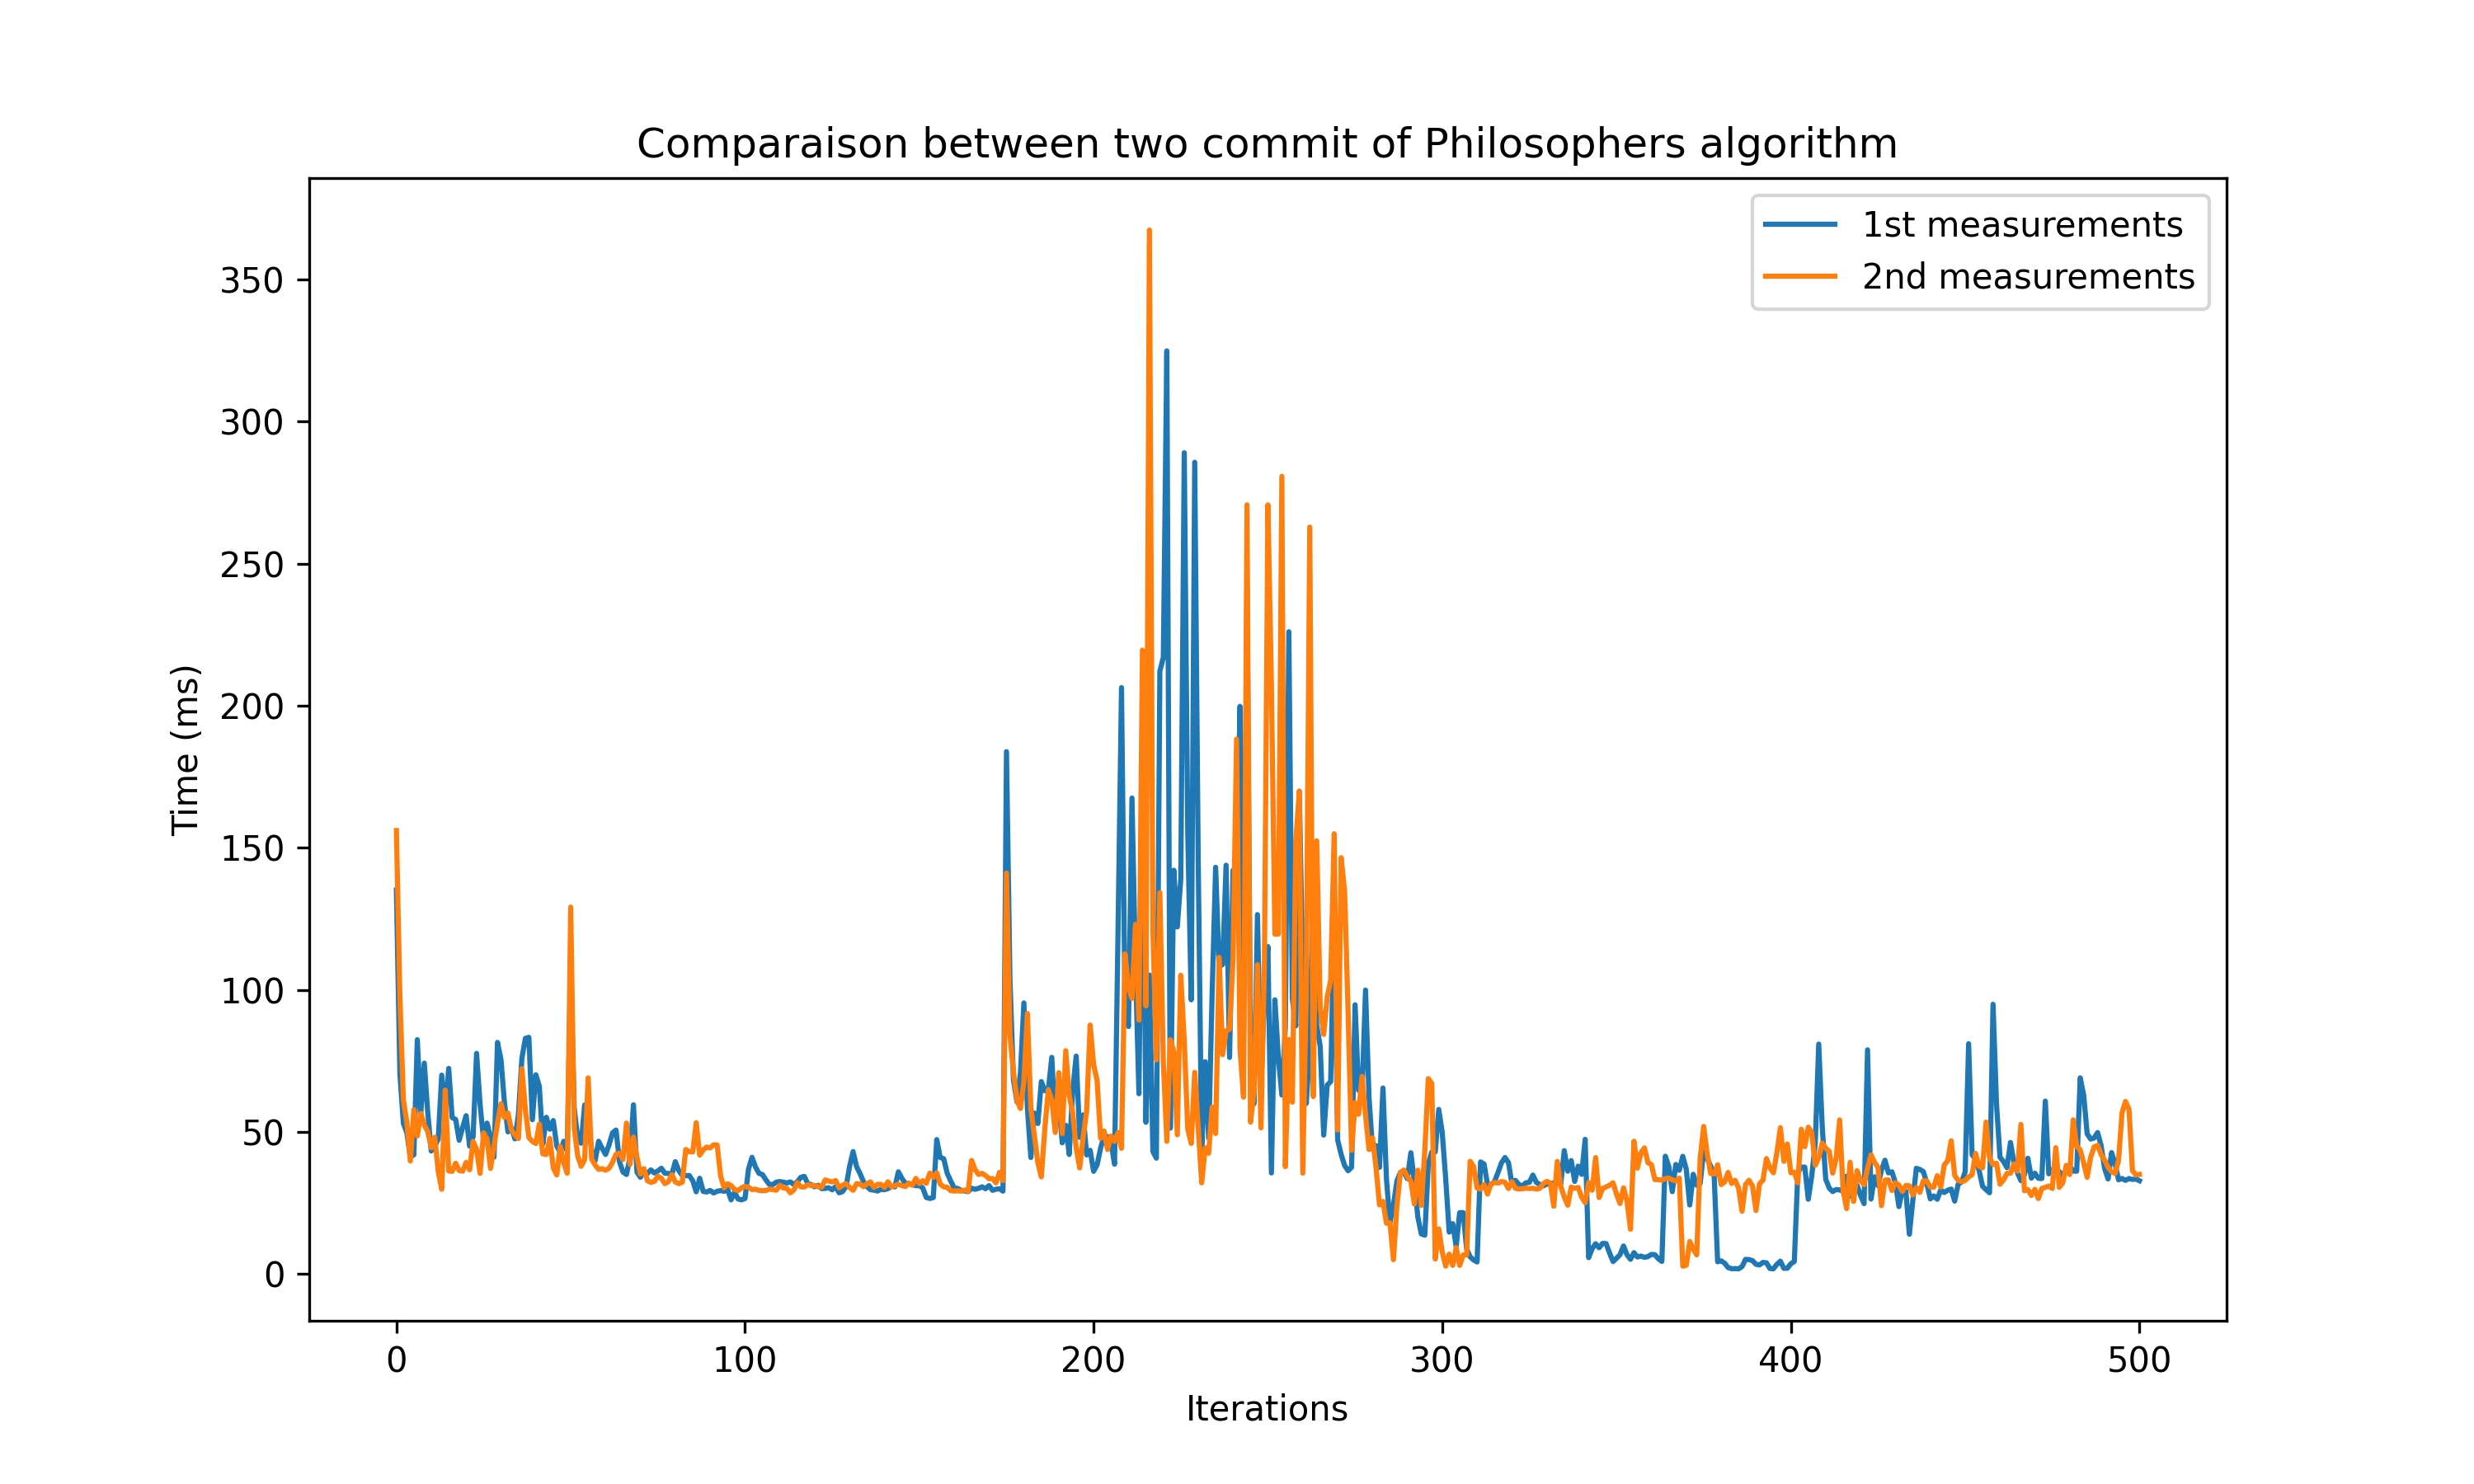
\includegraphics[width=8cm]{assets/plot_Philosophers_42.533000000000015.png}
\end{figure}


\section{August 3 - August 10}

Starting writing the introduction and review the warmup paper, I first wanted to improve the changepoint analysis, but I didn't have time, so i abandoned this part. I just make the adaptation of the algorithm.

\section{August 10 - August 17}

I fixed some bugs.

I made the documentation and the HTML file for the corpus for the API and the code.

The api is publicly deployed on my server but can be deployed eveywhere using docker
\url{https://api.rebench.vatoth.dev}

\section{August 17 - August 24}

I started to write the review sections of algorithms and reported the result.
I also wrote the engineering process of the dissertation about the work that is done on it.

\section{August 24 - August 30}

I wrote the evaluation and conclusion and reformated a bit of the dissertation.

\section{August 30 - September 6}

Finishing the dissertation checking grammar and the overall flow of the dissertation

\end{document}

